%% Préambule
\documentclass[10pt, french]{article}
% !TEX encoding = UTF-8 Unicode
% LaTeX Preamble for all cheatsheets
% Author : Gabriel Crépeault-Cauchon

% HOW-TO : copy-paste this file in the same directory as your .tex file, and add in your preamble the next command right after you have specified your documentclass : 
% \input{preamble-cheatsht.tex}
% ---------------------------------------------
% ---------------------------------------------

% Extra note : this preamble creates document that are meant to be used inside the multicols environment. See the documentation on internet for further information.

%% -----------------------------
%% Encoding packages
%% -----------------------------
\usepackage[utf8]{inputenc}
\usepackage[T1]{fontenc}
\usepackage{babel}
\usepackage{lmodern}

%% -----------------------------
%% Variable definition
%% -----------------------------
\def\auteur{Gabriel Crépeault-Cauchon / Nicholas Langevin}
\def\BackgroundColor{white}

%% -----------------------------
%% Margin and layout
%% -----------------------------
% Determine the margin for cheatsheet
\usepackage[landscape, hmargin=1cm, vmargin=1.7cm]{geometry}
\usepackage{multicol}

% Remove automatic indentation after section/subsection title.
\setlength{\parindent}{0cm}

% Save space in cheatsheet by removing space between align environment and normal text.
\usepackage{etoolbox}
\newcommand{\zerodisplayskips}{%
  \setlength{\abovedisplayskip}{0pt}%
  \setlength{\belowdisplayskip}{0pt}%
  \setlength{\abovedisplayshortskip}{0pt}%
  \setlength{\belowdisplayshortskip}{0pt}}
\appto{\normalsize}{\zerodisplayskips}
\appto{\small}{\zerodisplayskips}
\appto{\footnotesize}{\zerodisplayskips}

%% -----------------------------
%% URL and links
%% -----------------------------
\usepackage{hyperref}
\hypersetup{colorlinks = true, urlcolor = gray!70!white, linkcolor = black}

%% -----------------------------
%% Document policy (uncomment only one)
%% -----------------------------
%	\usepackage{concrete}
	\usepackage{mathpazo}
%	\usepackage{frcursive} %% permet d'écrire en lettres attachées
%	\usepackage{aeguill}
%	\usepackage{mathptmx}
%	\usepackage{fourier} 

%% -----------------------------
%% Math configuration
%% -----------------------------
\usepackage[fleqn]{amsmath}
\usepackage{amsthm,amssymb,latexsym,amsfonts}
\usepackage{empheq}
\usepackage{numprint}
\usepackage{dsfont} % Pour avoir le symbole du domaine Z

% Mathematics shortcuts

\newcommand{\reels}{\mathbb{R}}
\newcommand{\entiers}{\mathbb{Z}}
\newcommand{\naturels}{\mathbb{N}}
\newcommand{\eval}{\biggr \rvert}
\usepackage{cancel}
\newcommand{\derivee}[1]{\frac{\partial}{\partial #1}}
\newcommand{\prob}[1]{\Pr \left( #1 \right)}
\newcommand{\esp}[1]{\mathrm{E} \left[ #1 \right]} % espérance
\newcommand{\variance}[1]{\mathrm{Var} \left( #1   \right)}
\newcommand{\covar}[1]{\mathrm{Cov} \left( #1   \right)}
\newcommand{\laplace}{\mathcal{L}}
\newcommand{\deriv}[2][]{\frac{\partial^{#1}}{\partial #2^{#1}}}
\newcommand{\e}[1]{\mathrm{e}^{#1}}
\newcommand{\te}[1]{\text{exp}\left\{#1\right\}}
\DeclareMathSymbol{\shortminus}{\mathbin}{AMSa}{"39}



% To indicate equation number on a specific line in align environment
\newcommand\numberthis{\addtocounter{equation}{1}\tag{\theequation}}

%
% Actuarial notation packages
%
\usepackage{actuarialsymbol}
\usepackage{actuarialangle}

%
% Matrix notation for math symbols (\bm{•})
%
\usepackage{bm}
% Matrix notation variable (bold style)
\newcommand{\matr}[1]{\mathbf{#1}}



%% -----------------------------
%% tcolorbox configuration
%% -----------------------------
\usepackage[most]{tcolorbox}
\tcbuselibrary{xparse}
\tcbuselibrary{breakable}

%%
%% Coloured box "definition" for definitions
%%
\DeclareTColorBox{definition}{ o }				% #1 parameter
{
	colframe=blue!60!green,colback=blue!5!white, % color of the box
	breakable, 
	pad at break* = 0mm, 						% to split the box
	title = {#1},
	after title = {\large \hfill \faBook},
}
%%
%% Coloured box "definition2" for definitions
%%
\DeclareTColorBox{definitionNOHFILL}{ o }				% #1 parameter
{
	colframe=blue!60!green,colback=blue!5!white, % color of the box
	pad at break* = 0mm, 						% to split the box
	title = {#1},
	before title = {\faBook \quad },
	breakable
}


%%
%% Coloured box "algo" for algorithms
%%
\newtcolorbox{algo}[ 1 ]
{
	colback = blue!5!white,
	colframe = blue!75!black,
	title=#1,
	fonttitle = \bfseries,
	breakable
}
%%
%% Coloured box "conceptgen" for points adding to a concept's deifintion
%%
\newtcolorbox{conceptgen}[ 1 ]
{
	breakable,
	colback = beaublue,
	colframe = airforceblue,
	title=#1,
	fonttitle = \bfseries
}
%%
%% Coloured box "probch3" pour formules relatives au 3ème chapitre de prob
%%
\newtcolorbox{probch3}[ 1 ]
{
	colback = ruddypink,
	colframe = burgundy,
	fonttitle = \bfseries,	
	breakable,
	title=#1
}
%%
%% Coloured box "formula" for formulas
%%
\newtcolorbox{formula}[ 1 ]
{
	colback = green!5!white,
	colframe = green!70!black,
	breakable,
	fonttitle = \bfseries,
	title=#1
}
%%
%% Coloured box "formula" for formulas
%%
\DeclareTColorBox{algo2}{ o }
{
	enhanced,
	title = #1,
	colback=blue!5!white,	
	colbacktitle=blue!75!black,
	fonttitle = \bfseries,
	breakable,
	boxed title style={size=small,colframe=arsenic} ,
	attach boxed title to top center = {yshift=-3mm,yshifttext=-1mm},
}
%%
%% Coloured box "examplebox" for formulas
%%
\newtcolorbox{examplebox}[ 1 ]
{
	colback = lightmauve,
	colframe = antiquefuchsia,
	breakable,
	fonttitle = \bfseries,title=#1
}
%%
%% Coloured box "rappel" pour rappel de formules
%%
\newtcolorbox{rappel}[ 1 ]
{
	colback = ashgrey,
	colframe = arsenic,
	breakable,
	fonttitle = \bfseries,title=#1
}
%%
%% Coloured box "rappel" pour rappel de formules
%%
\DeclareTColorBox{rappel_enhanced}{ o }
{
	enhanced,
	title = #1,
	colback=ashgrey, % color of the box
%	colframe=blue(pigment),
%	colframe=arsenic,	
	colbacktitle=arsenic,
	fonttitle = \bfseries,
	breakable,
	boxed title style={size=small,colframe=arsenic} ,
	attach boxed title to top center = {yshift=-3mm,yshifttext=-1mm},
}
%%
%% Coloured box "notation" for notation and terminology
%%
\DeclareTColorBox{distributions}{ o }			% #1 parameter
{
	enhanced,
	title = #1,
	colback=gray(x11gray), % color of the box
%	colframe=blue(pigment),
	colframe=arsenic,	
	colbacktitle=aurometalsaurus,
	fonttitle = \bfseries,
	boxed title style={size=small,colframe=arsenic} ,
	attach boxed title to top center = {yshift=-3mm,yshifttext=-1mm},
	breakable
%	left=0pt,
%  	right=0pt,
%    box align=center,
%    ams align*
%  	top=-10pt
}

%% -----------------------------
%% Graphics and pictures
%% -----------------------------
\usepackage{graphicx}
\usepackage{pict2e}
\usepackage{tikz}

%% -----------------------------
%% insert pdf pages into document
%% -----------------------------
\usepackage{pdfpages}

%% -----------------------------
%% Color configuration
%% -----------------------------
\usepackage{color, soulutf8, colortbl}


%
%	Colour definitions
%
\definecolor{blue(munsell)}{rgb}{0.0, 0.5, 0.69}
\definecolor{blue(matcha)}{rgb}{0.596, 0.819, 1.00}
\definecolor{blue(munsell)-light}{rgb}{0.5, 0.8, 0.9}
\definecolor{bleudefrance}{rgb}{0.19, 0.55, 0.91}
\definecolor{blizzardblue}{rgb}{0.67, 0.9, 0.93}
\definecolor{bondiblue}{rgb}{0.0, 0.58, 0.71}
\definecolor{blue(pigment)}{rgb}{0.2, 0.2, 0.6}
\definecolor{bluebell}{rgb}{0.64, 0.64, 0.82}
\definecolor{airforceblue}{rgb}{0.36, 0.54, 0.66}
\definecolor{beaublue}{rgb}{0.74, 0.83, 0.9}
\definecolor{cobalt}{rgb}{0.0, 0.28, 0.67}	% nice light blue-ish
\definecolor{blue_rectangle}{RGB}{83, 84, 244}		% ACT-2004
\definecolor{indigo(web)}{rgb}{0.29, 0.0, 0.51}	% purple-ish
\definecolor{antiquefuchsia}{rgb}{0.57, 0.36, 0.51}	%	pastel dark purple ish
\definecolor{darkpastelpurple}{rgb}{0.59, 0.44, 0.84}
\definecolor{gray(x11gray)}{rgb}{0.75, 0.75, 0.75}
\definecolor{aurometalsaurus}{rgb}{0.43, 0.5, 0.5}
\definecolor{ruddypink}{rgb}{0.88, 0.56, 0.59}
\definecolor{pastelred}{rgb}{1.0, 0.41, 0.38}		
\definecolor{lightmauve}{rgb}{0.86, 0.82, 1.0}
\definecolor{azure(colorwheel)}{rgb}{0.0, 0.5, 1.0}
\definecolor{darkgreen}{rgb}{0.0, 0.2, 0.13}			
\definecolor{burntorange}{rgb}{0.8, 0.33, 0.0}		
\definecolor{burntsienna}{rgb}{0.91, 0.45, 0.32}		
\definecolor{ao(english)}{rgb}{0.0, 0.5, 0.0}		% ACT-2003
\definecolor{amber(sae/ece)}{rgb}{1.0, 0.49, 0.0} 	% ACT-2004
\definecolor{green_rectangle}{RGB}{131, 176, 84}		% ACT-2004
\definecolor{red_rectangle}{RGB}{241,112,113}		% ACT-2004
\definecolor{amethyst}{rgb}{0.6, 0.4, 0.8}
\definecolor{amethyst-light}{rgb}{0.6, 0.4, 0.8}
\definecolor{ashgrey}{rgb}{0.7, 0.75, 0.71}			% dark grey-black-ish
\definecolor{arsenic}{rgb}{0.23, 0.27, 0.29}			% light green-beige-ish gray
\definecolor{amaranth}{rgb}{0.9, 0.17, 0.31}
\definecolor{brickred}{rgb}{0.8, 0.25, 0.33}
\definecolor{pastelred}{rgb}{1.0, 0.41, 0.38}

%
% Useful shortcuts for coloured text
%
\newcommand{\orange}{\textcolor{orange}}
\newcommand{\red}{\textcolor{red}}
\newcommand{\cyan}{\textcolor{cyan}}
\newcommand{\blue}{\textcolor{blue}}
\newcommand{\green}{\textcolor{green}}
\newcommand{\purple}{\textcolor{magenta}}
\newcommand{\yellow}{\textcolor{yellow}}

%% -----------------------------
%% Enumerate environment configuration
%% -----------------------------
%
% Custum enumerate & itemize Package
%
\usepackage{enumitem}
%
% French Setup for itemize function
%
\frenchbsetup{StandardItemLabels=true}
%
% Change default label for itemize
%
\renewcommand{\labelitemi}{\faAngleRight}


%% -----------------------------
%% Tabular column type configuration
%% -----------------------------
\newcolumntype{C}{>{$}c<{$}} % math-mode version of "l" column type
\newcolumntype{L}{>{$}l<{$}} % math-mode version of "l" column type
\newcolumntype{R}{>{$}r<{$}} % math-mode version of "l" column type
\newcolumntype{f}{>{\columncolor{green!20!white}}p{1cm}}
\newcolumntype{g}{>{\columncolor{green!40!white}}m{1.2cm}}
\newcolumntype{a}{>{\columncolor{red!20!white}$}p{2cm}<{$}}	% ACT-2005
% configuration to force a line break within a single cell
\usepackage{makecell}


%% -----------------------------
%% Fontawesome for special symbols
%% -----------------------------
\usepackage{fontawesome}

%% -----------------------------
%% Section Font customization
%% -----------------------------
\usepackage{sectsty}
\sectionfont{\color{\SectionColor}}
\subsectionfont{\color{\SubSectionColor}}

%% -----------------------------
%% Footer/Header Customization
%% -----------------------------
\usepackage{lastpage}
\usepackage{fancyhdr}
\pagestyle{fancy}

%
% Header
%
\fancyhead{} 	% Reset
\fancyhead[L]{Aide-mémoire pour~ \cours ~(\textbf{\sigle})}
\fancyhead[R]{\auteur}

%
% Footer
%
\fancyfoot{}		% Reset
\fancyfoot[R]{\thepage ~de~ \pageref{LastPage}}
\fancyfoot[L]{\href{https://github.com/ressources-act/Guide_de_survie_en_actuariat}{\faGithub \ ressources-act/Guide de survie en actuariat}}
%
% Page background color
%
\pagecolor{\BackgroundColor}




%% END OF PREAMBLE
% ---------------------------------------------
% ---------------------------------------------
\usepackage{array, multirow}
\usepackage{booktabs}
\usepackage{eurosym}
\usepackage{graphicx}
\graphicspath{{../figure/}}
\setlist{leftmargin=*}

%% -----------------------------
%% Préambule
%% -----------------------------
\def\BackgroundColor{white}
\def\SectionColor{teal!90!black}
\def\SubSectionColor{teal!45!black}
\def\SubSubSectionColor{armygreen}
\def\cours{Compléments de mathématiques}
\def\sigle{ACT-1003}


%% -----------------------------
%%	Feuille basée sur 
\begin{document}
\begin{center}
	\textsc{\Large Contributeurs}\\[0.5cm] 
%%
\end{center}
\begin{contrib}{ACT-1003\: Compléments de mathématiques}
\begin{description}
	\item[aut., cre.] Félix Cournoyer
	\item[src.] Ilie Radu Mitric
\end{description}
\end{contrib}
%% -----------------------------
\newpage

\raggedcolumns

\begin{multicols*}{2}

\section{Rappels}

\begin{conceptgen_enhanced}[Propriétés des limites]
\begin{itemize}
  \item $\lim_{x \to a}  (f(x) \pm g(x)) = \lim_{x \to a} f(x) \pm \lim_{x \to a} g(x)$ 
  \item $\lim_{x\to a} k*f(x) = k*\lim_{x\to a} f(x)$
  \item $\lim_{x\to a} (f(x)g(x)) = \lim_{x\to a} f(x)*\lim_{x\to a} g(x)$
  \item $\lim_{x\to a} \frac{f(x)}{g(x)} = \frac{\lim_{x\to a} f(x)}{\lim_{x\to a} g(x)}$
  \item $\lim_{x\to a} (f(x))^{n} = (\lim_{x\to a} f(x))^{n}$
  \item $\lim_{x\to a} \log_b (x) = \log_b{a} \iff a > 0$
  \item $\lim_{x\to \infty} \log_b (x) = \hspace{0.35cm}\infty \iff b > 1, \hspace{0.5cm}=-\infty \iff 0 < b < 1$
  \item $\lim_{x\to 0^{+}} \log_b (x) = -\infty \iff b > 1, \hspace{0.5cm}=\infty \iff 0 < b < 1$
\end{itemize}
\end{conceptgen_enhanced}

\begin{conceptgen_enhanced}[Opérations avec les $\infty$]
\begin{itemize}
 \item $k \pm \infty = \pm \infty$
 \item $\pm \infty * \pm \infty = \pm \infty$
 \item $k * \pm \infty = \pm \infty$
 \item $\frac{k}{\pm \infty} = 0$
 \item $\frac{k}{0^{+}} = \infty$, $\frac{k}{0^{-}} = -\infty$, pour k > 0
\end{itemize}
\end{conceptgen_enhanced}

\section{Fonctions}

\begin{definitionNOHFILL}[Caractéristiques de fonctions]
Il existe trois caractéristiques pour une fonction donnée : la surjectivité, l'injectivité et la bijectivité.\\

Lorsque tous les y d'une fonction, c'est-à-dire chaque élément de son image, sont tous reliés à au moins un x, la fonction est dite surjective. Par exemple, la fonction $x^{2}$ n'est pas surjective car y=-1 n'a pas de x dans les réels. Si on limite toutefois l'image aux réels positifs, la fonction devient surjective, car chaque y des réels positifs ont au moins un x correspondant.\\

Lorsque tous les y d'une fonction ne sont reliés qu'à un seul x, la fonction est dite injective. En reprenant $x^{2}$, on peut démontrer qu'elle n'est pas injective : $x^{2}=(-x)^{2}$. Toutefois, 2x est injective car il n'existe pas deux x pouvant donner le même y.\\

La fonction est bijective lorsqu'elle est à la fois bijective et injective, ce qui veut dire que chaque y de la fonction ne possède qu'un seul x. En reprenant 2x, on peut démontrer sa bijectivité : chaque y possède un x dans les réels. La fonction étant aussi injective, elle devient alors bijective.
\end{definitionNOHFILL}

\begin{definitionNOHFILL}[Racines réelles]
On peut identifier les racines réelles à l'aide d'un calcul simple. Si on a la fonction $ x^{3}-3x^{2}-10x+24 $, on doit utiliser la fonction suivante : \\
  \begin{equation*}
%% Difficulté à enlever l'italique et às séparer les mots dans la fraction
			\pm \frac{Facteurs positifs de a_{0}}{Facteurs positifs de a_{k}}
	\end{equation*}
Le numérateur serait 24 et le dénominateur serait 1 (car $24x^{0}$ et $1x^{3}$). Les racines de la fonction sont donc $\in \{ {\pm 1; \pm 2; \pm 3; \pm 4; \pm 6; \pm 8; \pm 12; \pm 24} \}$. Il faut ensuite essayer les chiffres de l'ensemble de la fonction. Par exemple, en ayant x=2, la fonction donne 0. En divisant la fonction par (x-2), il reste $x^{2}-x-12$. On peut encore essayer avec les racines du départ et on verrait qu'en ayant x=-3, la fonction donne 0, ou on peut déjà voir qu'il reste (x+3)(x-4).
\end{definitionNOHFILL}

\begin{definitionNOHFILL}[Fonctions inverses]
Pour obtenir une fonction inverse, il faut avoir une fonction bijective sur l'intervalle donné dans l'énoncé. Par la suite, on isole x dans la fonction et on remplace x par $f^{-1}(x)$ et y par x. Pour reprendre l'exemple plus haut :
  \begin{align*}
  f(x) = x^{2}
  \end{align*}
On peut trouver l'inverse lorsque les intervalles sont de $[ 0, \infty [ \rightarrow [ 0, \infty [$ étant donné la bijectivité sur cet intervalle. En isolant x, on a la fonction $\sqrt{y} = x$ et on remplace les variables. On obtient $\sqrt{x} = f^{-1}(x)$ pour les intervalles $[ 0, \infty [ \rightarrow [ 0, y [$. 
\end{definitionNOHFILL}

\begin{definitionNOHFILL}[Fonctions monotones]
% Il serait intéressant d'insérer des graphiques
Il existe quatre types de fonctions monotones. \\
La première la fonction dite non-décroissante; elle augmente sans arrêt, mais peut avoir un plateau ($f(x_{1}) \leq f(x_{2})$). \\
Il y a la fonction strictement croissante, qui s'apparente à la première, mais qui ne peut avoir de plateaux ($f(x_{1}) < f(x_{2})$). On peut penser à une fonction linéaire à pente positive pour se l'imaginer. Une fonction qui est strictement croissante est donc aussi non-décroissante. Une fonction en escalier avec une "pente positive" serait par exemple une fonction non-décroissante, mais pas strictement croissante avec ses plateaux.\\
Il existe aussi la fonction non-croissante, qui se veut une fonction décroissante sur son domaine, mais qui peut avoir un plateau ($f(x_{1}) \geq f(x_{2})$). \\
Pour finir, il y a aussi la fonction strictement décroissante, où il ne peut y avoir de plateaux ($f(x_{1}) > f(x_{2})$). On peut penser à une fonction linéaire à pente négative pour se l'imaginer. Une fonction qui est strictement décroissante est donc automatiquement une fonction non-croissante.
\end{definitionNOHFILL}

\section{Limites}
%% connaissance limitée avec les limites epsilon et delta, à revoir

\begin{rappel}{Les indéterminations}
  Une limite est dite indéterminée lorsque son résultat est un calcul utilisant les infinis. Les principales indéterminations sont les suivantes :
  \begin{itemize}
    \item $\frac{0}{0}$
    \item $\pm \frac{\infty}{\infty}$
    \item $\infty - \infty$
    \item $0 \cdot \infty$
    \item $1^{\infty}$
    \item $0^{0}$
    \item $\infty^{0}$
  \end{itemize}
\end{rappel}

\begin{rappel}{Théorème du sandwich}
Nous avons au départ:
  \begin{align*}
  \lim_{x \to a}  f(x) = \lim_{x \to a} g(x) = L
  \end{align*}
\\Nous avons aussi la fonction h suivante :
  \begin{align*}
    f(x) \leq h(x) \leq g(x)
  \end{align*}
  Le but du théorème est alors de trouver la valeur de la limite de h, comme on peut voir par cette image :\\
% j'essaye de rentrer la figure
%  \begin{figure}
%    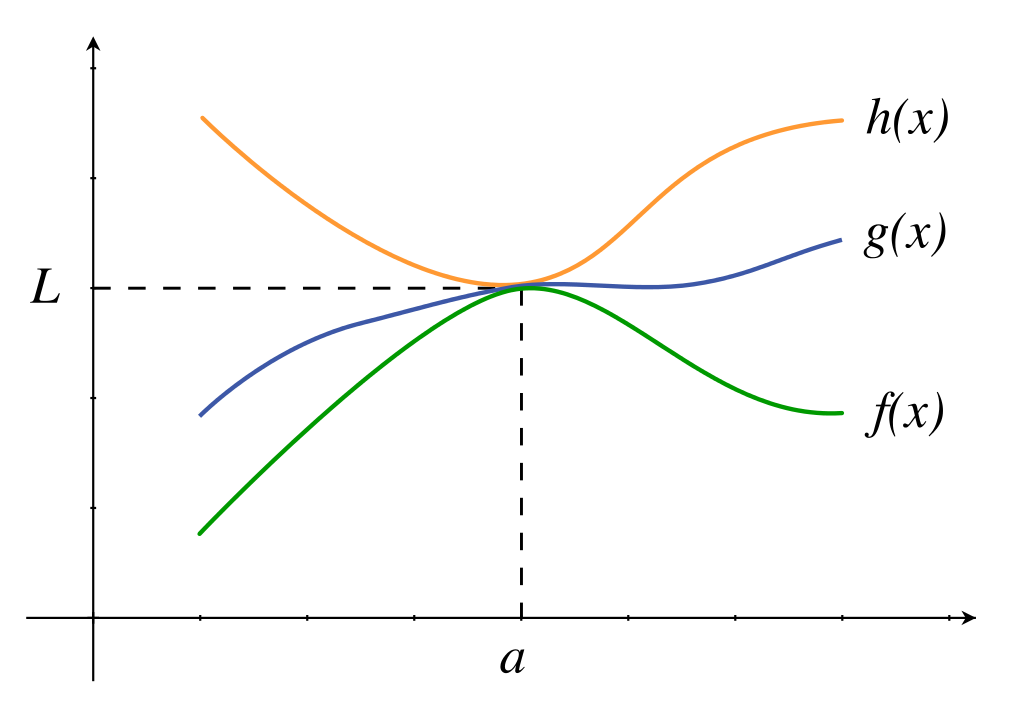
\includegraphics[width=\textwidth]{Sandwich.png}
%  \end{figure}
Une limite classique pour démontrer le théorème est $\lim_{x \to \infty} \frac{\sin(x)}{x}$. Elle représente notre h que nous désirons isoler. Nous devons nous retrouver avec cette limite encadrée de deux fonctions calculables. Ici, la fonction sinus est difficile à calculer à l'infini. Nous sommes toutefois certain que $\sin(x)$ donne un résultat entre -1 et 1 :

  \begin{align*}
    -1 \leq \sin(x) \leq 1
  \end{align*}

Nous commencons donc à voir que la fonction centrale ressemble à la fonction h de départ. Nous divisons donc le tout par x :
\begin{align*}
    \frac{-1}{x} \leq \frac{\sin(x)}{x} \leq \frac{1}{x}
  \end{align*}

Nous retrouvons donc la fraction centrale h. En évaluant à l'infini le sandwich constitué de $\frac{-1}{x}$ et de $\frac{1}{x}$, nous obtenons 0 de part et d'autre du sandwich, ce qui signifie que le milieu doit aussi être égal à 0 pour que l'équation soit vraie.
\end{rappel}

\begin{rappel}{Limites avec une fonction composée}
  \begin{rappel}{La fonction composée}
  La fonction composée correspond à une fonction évaluée dont cette évaluation est utilisée pour une autre fonction. Par exemple, en considérant f comme étant la fonction $x^{2}$ et g étant 3x, la fonction (f $\circ$ g)(x) -à prononcer f rond g- évaluée avec x=5 donne 225. On peut le voir comme f(g(x)).
  \end{rappel}
  La fonction composée n'est pas vraiment affectée par les limites. Nous avons :
  \begin{itemize}
    \item $\lim_{x \to a}  g(x) = b$ 
    \item $\lim_{x \to a}  (f \circ g) (x) = f(\lim_{x \to a}  g(x)) = f(b)$
  \end{itemize}
\end{rappel}

\begin{rappel}{Règle de L'Hospital}
En ayant une limite de la forme $\lim_{x \to a}  \frac{f(x)}{g(x)}$, on peut utiliser la règle de L'Hospital (la dérivée du numérateur et du dénominateur) seulement si la limite donne l'indétermination 0/0 ou $\pm \frac{\infty}{\infty}$. Visuellement, on obtient ceci lorsque la règle est applicable :
  \begin{align*}
    \lim_{x \to a}  \frac{f(x)}{g(x)}=\lim_{x \to a}  \frac{f'(x)}{g'(x)}
  \end{align*}
\end{rappel}

\begin{rappel}{Factorisation des limites}
Il est possible d'avoir une limite évaluée à l'infini qui donne $\frac{\infty}{\infty}$, ce qui est indéterminé. Pour   évaluer cette limite, on peut passer par la règle de L'Hospital, mais cela peut donner lieu à des dérivations successives et on obtient rien ou la limite est tout simplement difficile à dériver. Il y a toutefois une autre façon qui est assez simple, c'est-à-dire sortir l'élément qui a la puissance la plus élevée. Voici un exemple :
  \begin{itemize}
  \item $\lim_{x \to \infty} \frac{7*x^{4}-2*x+4}{2*x^{5}-3*x^{3}-11} = \frac{\infty}{\infty}$
  \item On peut toutefois sortir $x^{4}$ du numérateur et $x^{5}$ du dénominateur.
  \item $\lim_{x \to \infty} \frac{x^{4}*(7-\frac{2}{x^{3}}+\frac{4}{x^{4}})}{x^{5}*(2-\frac{3}{x^{2}}-\frac{11}{x^{5}})}     = \lim_{x \to \infty} \frac{7-\frac{2}{x^{3}}+\frac{4}{x^{4}}}{x*(2-\frac{3}{x^{2}}-\frac{11}{x^{5}})}$
  \end{itemize}
De ce qu'on a vu précédemment avec les opérations avec les $\infty$, le numérateur donne 7 et le dénominateur donne $2*\infty$, ce qui nous amène à la valeur de la limite qui est de 0.
\end{rappel}

\begin{rappel}{Utilisation du conjugué}
  \begin{rappel}{Le conjugué}
    Lorsqu'il y a un binôme de la forme $a-\sqrt{f(x)}$, son conjugué sera $a+\sqrt{f(x)}$. L'inverse est aussi vrai. Multiplier un binôme par son conjugué donne $a^{2}-f(x)$.
  \end{rappel}
  Nous avons la limite suivante :
  \begin{align*}
    \lim_{x \to 3} \frac{x^{2}-9}{1-\sqrt{x^{2}-8}}
  \end{align*}
  Lorsque l'on évalue la limite, on obtient 0/0, ce qui est indéterminé. Nous pouvons toutefois utiliser le conjugué :
  \begin{itemize}
  \item  $\lim_{x \to 3} \frac{x^{2}-9}{1-\sqrt{x^{2}-8}} \cdot \frac{1+\sqrt{x^{2}-8}}{1+\sqrt{x^{2}-8}}$
  \item $\lim_{x \to 3} \frac{(x^{2}-9)(1+\sqrt{x^{2}-8})}{1-x^{2}+8} = \lim_{x \to 3} \frac{(x^{2}-9)(1+\sqrt{x^{2}-8})}{9-x^{2}}$
  \item $-\lim_{x \to 3} 1+\sqrt{x^{2}-8} = -2$
  \end{itemize}
  Le conjugué permet donc de se débarrasser d'un élément, que ce soit au numérateur ou au dénominateur. Dans l'exemple, nous avions exactement le bon terme, mais il faudra parfois utiliser la différence de carrés pour simplifier le tout.
\end{rappel}

\begin{rappel}{Continuité}
  Si une limite existe au point a et que celle-ci n'est pas égale à l'infini, la fonction est continue au point a et est égale à la fonction évaluée en ce point. Par exemple, $-1/\lvert{x}\rvert$, ne serait pas continue en 0. Bien que la limite existe, elle est de $-\infty$, ce qui infirme sa continuité.\\
  Rappel 1 : pour qu'une fonction soit continue, il faut aussi que la fonction évaluée en a soit égale à la valeur de la limite en a. Cela fait juste confirmer l'exemple : f(0) n'avait pas de valeur, alors que la limite est de $-\infty$. Les exemples courants en ce sens sont des fonctions définies par parties.\\
  Rappel 2 : la limite doit être égale de part et d'autres du point a pour être définie. Par exemple, $\lim_{x \to 0} 1/x$ n'est pas définie, car en $0^{-}$, la fonction vaut $-\infty$ et en $0^{+}$, la fonction vaut $\infty$ et $-\infty \ne \infty$.
  \begin{rappel}{Résumé}
  Il y a deux conditions pour établir la continuité en un point a :
  \begin{itemize}
    \item $\lim_{x \to a} f(x)$ existe
    \item $\lim_{x \to a} f(x) = f(a)$, pourvu que f(a) existe et $\ne \pm \infty$
   \end{itemize}
  \end{rappel}
\end{rappel}

\begin{rappel}{Théorème des valeurs intermédiaires}
  Avec une fonction continue dans l'intervalle [a, b] et w un nombre situé entre f(a) et f(b), il doit exister au moins un nombre c tel que f(w)=c situé dans [a, b]. 
\end{rappel}

\section{La dérivée}

\begin{definitionNOHFILLsub}[Formules de binômes et rappels]
  \begin{itemize}
    \item $(a+b)^{2} = a^{2} + 2ab + b^{2}$
    \item $(a-b)^{2} = a^{2} - 2ab + b^{2}$
    \item $(a+b)^{3} = a^{3} + 3a^{2}b + 3ab^{2} + b^{3}$
    \item $(a-b)^{3} = a^{3} - 3a^{2}b + 3ab^{2} - b^{3}$
    \item $a^{n}+b^{n} = (a+b)(a^{n-1}-a{n-2}b+a^{n-3}b^{2}+ \dots -ab^{n-2}+b^{n-1}$
    \item $a^{n}-b^{n} = (a-b)(a^{n-1}+a{n-2}b+a^{n-3}b^{2}+ \dots +ab^{n-2}+b^{n-1}$
    \item $S_{n} = 1+r+r^{2}+ \dots +r^{n}=\frac{1-r^{n+1}}{1-r}$
    \item $S_{\infty} = \infty$ si r $\geq$ 1, $\varnothing$ si r $\leq$ -1, $\frac{1}{1-r}$ si $-1 < r < 1$
  \end{itemize}
\end{definitionNOHFILLsub}

\begin{definitionNOHFILLsub}[Définition de la dérivée]
  La dérivée en un point a est définie par la limite suivante :\\
  \begin{align*}
    f'(x)=\frac{d}{dx} f(x)=\lim_{h \to 0} \frac{f(a+h)-f(a)}{h}
  \end{align*}
  Plus h est petit, plus la mesure de la dérivée est précise. Avec un h de $0^{+}$, on obtient le taux de variation instantané, ce qui est la pente exacte au point a. On peut d'ailleurs obtenir les formules de dérivation en utilisant la formule de la définition.\\
  On parle de dérivée à gauche lorsque $h \to 0^{-}$ et de dérivée à droite lorsque $h \to 0^{+}$.
  
\end{definitionNOHFILLsub}

\end{multicols*}
%% -----------------------------
\end{document}
